%% This is file `elsarticle-template-1-num.tex',
%%
%% Copyright 2009 Elsevier Ltd
%%
%% This file is part of the 'Elsarticle Bundle'.
%% ---------------------------------------------
%%
%% It may be distributed under the conditions of the LaTeX Project Public
%% License, either version 1.2 of this license or (at your option) any
%% later version.  The latest version of this license is in
%%    http://www.latex-project.org/lppl.txt
%% and version 1.2 or later is part of all distributions of LaTeX
%% version 1999/12/01 or later.
%%
%% The list of all files belonging to the 'Elsarticle Bundle' is
%% given in the file `manifest.txt'.
%%
%% Template article for Elsevier's document class `elsarticle'
%% with numbered style bibliographic references
%%
%% $Id: elsarticle-template-1-num.tex 149 2009-10-08 05:01:15Z rishi $
%% $URL: http://lenova.river-valley.com/svn/elsbst/trunk/elsarticle-template-1-num.tex $
%%
\documentclass[12pt]{elsarticle}

%% Use the option review to obtain double line spacing
%% \documentclass[preprint,review,12pt]{elsarticle}

%% Use the options 1p,twocolumn; 3p; 3p,twocolumn; 5p; or 5p,twocolumn
%% for a journal layout:
%% \documentclass[final,1p,times]{elsarticle}
%% \documentclass[final,1p,times,twocolumn]{elsarticle}
%% \documentclass[final,3p,times]{elsarticle}
%% \documentclass[final,3p,times,twocolumn]{elsarticle}
%% \documentclass[final,5p,times]{elsarticle}
%% \documentclass[final,5p,times,twocolumn]{elsarticle}

%% if you use PostScript figures in your article
%% use the graphics package for simple commands
%% \usepackage{graphics}
%% or use the graphicx package for more complicated commands
%% \usepackage{graphicx}
%% or use the epsfig package if you prefer to use the old commands
%% \usepackage{epsfig}

%% The amssymb package provides various useful mathematical symbols

\usepackage[paper=a4paper,
includefoot, % Uncomment to put page number above margin
marginparwidth=30.5mm,    % Length of section titles
marginparsep=1.5mm,       % Space between titles and text
margin=25mm,              % 25mm margins
rmargin=0mm,
includemp]{geometry}


\usepackage{amssymb}

\usepackage{amssymb}
\usepackage{lineno}
\usepackage{amsmath}
\usepackage{amsfonts} % if you want blackboard bold symbols e.g. for real numbers
\usepackage{graphicx} % if you want to include jpeg or pdf pictures
\DeclareGraphicsExtensions{.pdf,.png,.jpg}
\usepackage{mathtools}

%% The amsthm package provides extended theorem environments
%% \usepackage{amsthm}

%% The lineno packages adds line numbers. Start line numbering with
%% \begin{linenumbers}, end it with \end{linenumbers}. Or switch it on
%% for the whole article with \linenumbers after \end{frontmatter}.
\usepackage{lineno}

%% natbib.sty is loaded by default. However, natbib options can be
%% provided with \biboptions{...} command. Following options are
%% valid:

%%   round  -  round parentheses are used (default)
%%   square -  square brackets are used   [option]
%%   curly  -  curly braces are used      {option}
%%   angle  -  angle brackets are used    <option>
%%   semicolon  -  multiple citations separated by semi-colon
%%   colon  - same as semicolon, an earlier confusion
%%   comma  -  separated by comma
%%   numbers-  selects numerical citations
%%   super  -  numerical citations as superscripts
%%   sort   -  sorts multiple citations according to order in ref. list
%%   sort&compress   -  like sort, but also compresses numerical citations
%%   compress - compresses without sorting
%%
%% \biboptions{comma,round}

% \biboptions{}


\journal{}

\begin{document}
	
	\begin{frontmatter}
		
		%% Title, authors and addresses
		
		%% use the tnoteref command within \title for footnotes;
		%% use the tnotetext command for the associated footnote;
		%% use the fnref command within \author or \address for footnotes;
		%% use the fntext command for the associated footnote;
		%% use the corref command within \author for corresponding author footnotes;
		%% use the cortext command for the associated footnote;
		%% use the ead command for the email address,
		%% and the form \ead[url] for the home page:
		%%
		%% \title{Title\tnoteref{label1}}
		%% \tnotetext[label1]{}
		%% \author{Name\corref{cor1}\fnref{label2}}
		%% \ead{email address}
		%% \ead[url]{home page}
		%% \fntext[label2]{}
		%% \cortext[cor1]{}
		%% \address{Address\fnref{label3}}
		%% \fntext[label3]{}
		
		\title{A Finite  Element Program for Potential flows}
		
		
		
		%% use optional labels to link authors explicitly to addresses:
		%% \author[label1,label2]{<author name>}
		%% \address[label1]{<address>}
		%% \address[label2]{<address>}
		
		\author{Karthik Reddy Lyathakula}
		
		\address{North Carolina State University, Raleigh,  United States}
		
		\begin{abstract}
			%% Text of abstract
			Finite element methods are based on variational principles which can be used to simulate any type of physics equations. The flexibility of these methods enables us to solve Multiphysics problems like fluid structural interaction, improve accuracy using higher-order schemes, and solve the physics equations on arbitrary meshes. In this project, FEM methods are used to solve potential flow problem to understand the implementation of FEM methods for flow simulation. In this work, linear elements with Lagrangian shape function is used to assemble the stiffness matrices and SGS method to solve a system of linear equations. FEM method is successfully implemented in two cases: Internal flow over a bump, External flow past a cylinder. Results from the first case are agreeing with the physical intuition. For the second case, a mesh independent study is conducted and compared with the exact solution to determine the order of accuracy. It was found that the scheme is the first-order accuracy as we are using linear elements.
		\end{abstract}
		
		
	\end{frontmatter}
	
	%%
	%% Start line numbering here if you want
	%%
	%%\linenumbers
	asdasdasds
	%% main text
	\section{Introduction}
	\label{S:1}
	
	Finite Element Methods (FEM) are methods that can be used to solve differential equations. By using these methods, any physics phenomena can be simulated if it can be described by mathematical equations. Understanding FEM methods will help in simulating physics phenomena and enable us to simulate Multiphysics problems, decrease computational effort, improve accuracy by using higher-order methods and it is suitable for arbitrary meshes. In this project, the FEM method is used to solve the potential flow problem to understand the implementation of FEM for fluid flow problems. 
	\section{Governing Equations}
	\label{S:2}
	Potential flows are the flow in which viscous effects are negligible and it is irrotational. Continuity and momentum equation for potential flow, which are also called Euler equations, are shown below:
	
	\begin{equation}
		\frac{\partial \rho}{\partial t}+\bigtriangledown \cdot(\rho \overrightarrow{u})=0
	\end{equation}
	
	\begin{equation}
		\frac{\partial (\rho \overrightarrow{u})}{\partial t}+\bigtriangledown \cdot (\rho \overrightarrow{u} \overrightarrow{u})+\bigtriangledown p =0
	\end{equation}
	At steady state, the time derivatives in the continuity and momentum equations will be zero. Irrotational flow condition is described by the equation:
	
	\begin{equation}
		\bigtriangledown \times \overrightarrow{u}=0
	\end{equation}
	For above equation to be true, there exist a scalar function $\phi$ such that $\overrightarrow{u}=\bigtriangledown \phi$. By substituting this equation in the continuity equation at steady state gives Potential flow equation.
	
	\begin{equation}\label{laplace equation}
		\bigtriangledown \cdot \bigtriangledown \phi=0.
	\end{equation}
	
	The momentum equation at steady state is given by 
	\begin{equation}
		\rho \overrightarrow{u} \cdot \bigtriangledown  \overrightarrow{u}+\bigtriangledown p=0
	\end{equation}
	Using the identity
	
	\begin{equation}
		\begin{gathered}
			\overrightarrow{u} \cdot \bigtriangledown\overrightarrow{u}= \left(\bigtriangledown \times \overrightarrow{u} \right) \times \overrightarrow{u} + \frac{ \overrightarrow{u} \cdot \overrightarrow{u}}{2}\\
			\left(\bigtriangledown \times \overrightarrow{u} \right)=0\\
			\overrightarrow{u} \cdot \bigtriangledown\overrightarrow{u}= \bigtriangledown \left(\frac{\overrightarrow{u} \cdot \overrightarrow{u}}{2}\right)\\
		\end{gathered}
	\end{equation}
	The momentum equations becomes Bernoulli equation.
	
	\begin{equation}
		\begin{gathered}
			\rho \bigtriangledown \left(\frac{\overrightarrow{u} \cdot \overrightarrow{u}}{2}\right)+\bigtriangledown p=0\\
			\rho \bigtriangledown \left(\frac{\overrightarrow{u} \cdot \overrightarrow{u}}{2}+p\right)=0\\
			\rho \frac{\overrightarrow{u} \cdot \overrightarrow{u}}{2}+p=const\\
		\end{gathered}
	\end{equation}
	The Bernoulli equation can be represented in potential function as:
	
	\begin{equation} \label{bernoli}
		\rho \frac{\bigtriangledown \overrightarrow{\phi} \cdot \bigtriangledown \overrightarrow{\phi}}{2}+p=const
	\end{equation}
	For a potential flow field, the equation \ref{laplace equation} is solved for the potential function and the function can be used to calculate the velocity and  pressure from Bernoulli equation \ref{bernoli}.
	\section{Finite Element Formulation for the potential equation}
	Finite element methods are based on variation principles which can discretize using finite dimension subspace and it is also suitable for arbitrary meshes (Structured and unstructured meshes)\newline
	\newline
	Introduce linear subspace
	\begin{equation}
		\begin{gathered}
			V=\{v:v\ is\ a\quad continuios\ function\ on\ Domain(\Omega)\\
			\quad \quad \quad \quad v_{,i}\ is\ piecewise\ continous\ and\ bounded\ on\ \Omega\
		\end{gathered}\}
	\end{equation}
	Here $v$ is also called as weight function. The starting point of FEM is to derive the weak formulation of the differential equation by multiplying the weight function on both sides of the differential equation and integration by parts. Weak formulation for potential flow equaiton \ref{laplace equation} is derived below.
	
	\begin{equation}
		\begin{gathered}
			\int_{\Omega} v (\bigtriangledown \cdot \bigtriangledown \phi)\ d \Omega=0\\
			\int_{\Omega} (\bigtriangledown \cdot v \bigtriangledown \phi-\bigtriangledown v \cdot \bigtriangledown\phi)\ d \Omega=0\\
			\int_{\Omega} \bigtriangledown \phi \cdot \bigtriangledown v \quad d \Omega =\int_{\Omega} \bigtriangledown \cdot v \bigtriangledown \phi \quad d \Omega\\
		\end{gathered}
	\end{equation} 
	Applying Divergence theorem gives on left hand of the above equation gives
	
	\begin{equation}
		\int_{\Omega} \bigtriangledown \phi \cdot \bigtriangledown v \quad d \Omega =\int_{\Gamma} v \left(\bigtriangledown \phi \cdot \overrightarrow{n}\right) d \Gamma
	\end{equation}
	Here $\Gamma$ is the boundary of the domain and $\left(\bigtriangledown \phi \cdot \overrightarrow{n}\right)$=g.\newline
	\newline
	Constructing a finite dimensional subspace $V_h$ of V:
	
	\begin{equation}
		\begin{gathered}
			T_h:\ Triangulization\ of\ \Omega\ by\ subdividing\ \Omega\\
			\quad into\ a\ set\ of\ non\ overlapping\ triangles\ (T_i)\\
			\Omega=U_{T\epsilon T_h}=T_1 U T_2 U T_3...............UT_h
		\end{gathered}
	\end{equation}
	$V_h$ is defined as 
	
	\begin{equation}
		\begin{gathered}
			V_h=\{v_h:v_h\ is\ a\ continous\ on\ \Omega_h \\
			\quad \quad \quad V_h|_T\ is\ linear\ for\ any\ T\varepsilon T_h \}
		\end{gathered}
	\end{equation}
	Dimension of $V_h$ is number of nodal points in the grid. The weak form in finite dimensional subspace $V_h$ of $V$
	is find $\phi \epsilon V_h$ such that 
	
	\begin{equation}
		\begin{gathered}
			\int_{{\Omega}_h} \bigtriangledown \phi_h \cdot \bigtriangledown v_h \quad d \Omega_h =\int_{\Gamma} v_h g d \Gamma
		\end{gathered}
	\end{equation}
	Introuduce the basis functions $(B_j \epsilon V_h)$.
	
	\begin{equation}
		\begin{gathered}
			\int_{{\Omega}_h} \bigtriangledown \phi_h \cdot \bigtriangledown B_j \quad d \Omega_h =\int_{\Gamma} B_j g d \Gamma \\ \quad for\quad  j=1,2,3......N
		\end{gathered}
	\end{equation}
	
	
	The $\phi_h$ is given by 
	
	\begin{equation}
		\phi_h=\sum\limits_{i=1}^{i=N} \phi_iB_i
	\end{equation}
	Here subscript 'i' indicates the node number and N is the maximum number of nodes in the mesh. $\phi_i$ is $\phi$ value at node 'i'. In this project, we are using the Galerkin method, where the basis function will be the same as the weight function. By introducing the $\phi_h$ we get a linear system of equations with N unknowns($\phi$).
	
	\begin{equation}
		\begin{gathered}
			\sum\limits_{i=1}^{i=N} \left(\int_{{\Omega}} \bigtriangledown B_i \cdot \bigtriangledown B_j \quad d \Omega \right) \phi_i =\int_{\Gamma} B_j g d \Gamma \\ \quad for\quad  j=1,2,3......N
		\end{gathered}
	\end{equation}
	The linear system of equations is of the form A$\phi$=b. Here A is the stiffness matrix of size NxN, b is the load matrix of size N x 1 and $\phi$ is the potential function values at node points. 
	
	\begin{equation}
		\begin{gathered}
			A_{ij}= \int_{\Omega_h} \bigtriangledown B_i \cdot \bigtriangledown B_j d \Omega\\
			b_j= \int_{\Gamma_h} g B_j d \Gamma
		\end{gathered}
	\end{equation}
	A is a symmetric matrix and positive definite. Hence the linear system of equations A$\phi$=b have unique solution
	
	In this project, the Langrangian shape function is used where the basis function at a node is defined in such a way that the function value is zero at its node point and non-zero at other nodes of the element. Basis functions are calculated using Barycentric coordinates from analytical geometry.
	
	\begin{figure}[h]
		\centering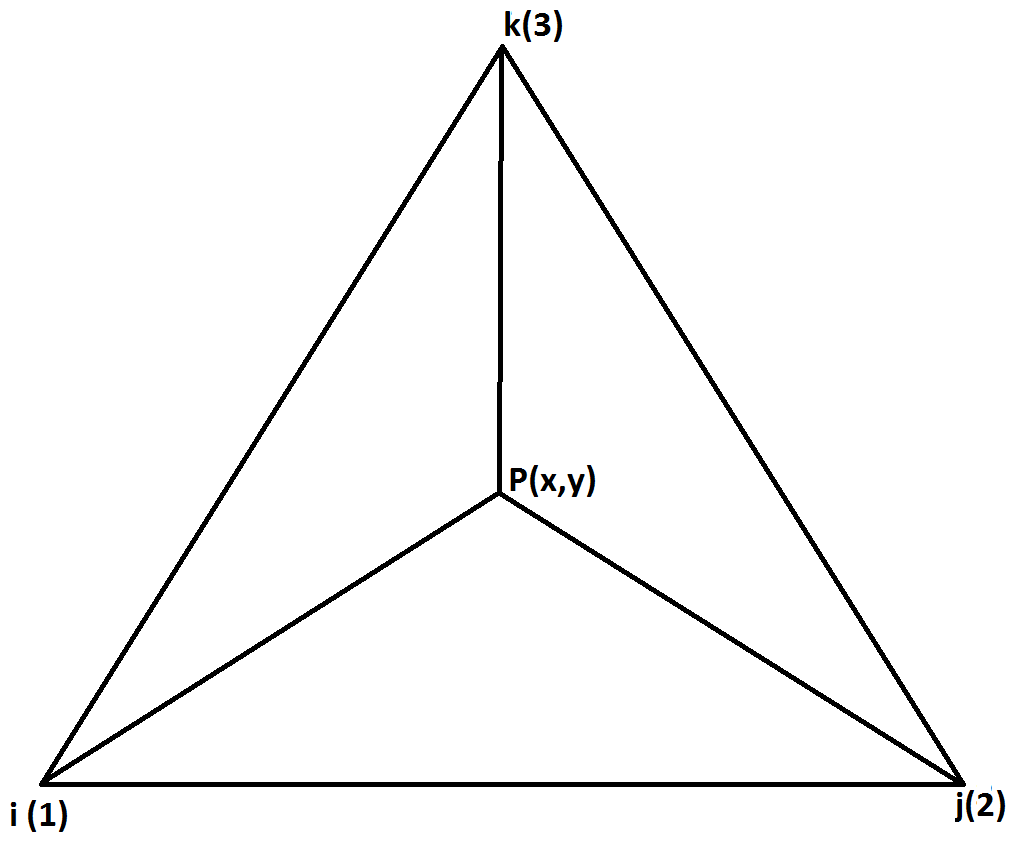
\includegraphics[width=0.5\linewidth]{figure_1.png}
		\caption{Bary Centric Coordinates}
	\end{figure}
	
	Functions $\lambda_1$,$\lambda_2$ and $\lambda_3$ are calculated from the areas of the triangle as shown below.
	
	\begin{equation}
		\begin{gathered}
			\lambda_1=\frac{\bigtriangleup P23}{\bigtriangleup123}\\
			\lambda_2=\frac{\bigtriangleup P31}{\bigtriangleup123}\\
			\lambda_3=\frac{\bigtriangleup P12}{\bigtriangleup123}\\
			\lambda_1+\lambda_2+\lambda_3=1
		\end{gathered}
	\end{equation}
	By calcualting the areas of the triangles we get the expression of $\lambda_i$ for each node of an elements as
	
	\begin{equation}
		\begin{gathered}
			\lambda_i=\frac{a_ix+b_iy+c_i}{D}\\
			for\ i=1,2,3\\
			a_i=y_j-y_k\\
			b_i=-x_j+x_k\\
			c_i=x_jy_k-x_ky_j\\
			D=c_1+c_2+c_3
		\end{gathered}
	\end{equation}
	In this project linear shapefunction is used and bases function will be $B_i=\lambda_i$. Using the basis function, the stiffness matrix and load matrix is assembelled.
	
	\section{Integration Method}
	After calculating system matrics, a linear set of algebraic equations need to solved as shown below
	
	\begin{equation}
		A \overrightarrow \phi = \overrightarrow b 
	\end{equation}\newline
	The size of the A matrix is NxN, where N is the number of nodes, and the size of  $ \overrightarrow b $ is Nx1. There are several ways to solve the system of equations which can be categorized into iterative and direct methods. In this project Symmetric Gauss-Seidel (SGS) method, one of the iterative methods is used.\newline
	\newline
	To solve the matrix system using iterative methods, matrix A is spitted into A = M+N, where M is the simple matrix and N is not a simple matrix. For SGS method, M is chosen as $(D-L)^-1D(D+L$.Before solving the system of matrices, they are arranged into the below form.
	
	\begin{equation}
		(M+N) {\overrightarrow \phi }_{k+1} = {\overrightarrow b}_{k} 
	\end{equation}
	
	\begin{equation}
		M {\overrightarrow \phi }_{k+1} = {\overrightarrow b}_{k} -(N) {\overrightarrow \phi }_k 
	\end{equation}
	
	\begin{equation}
		M {\overrightarrow \phi }_{k+1}- M {\overrightarrow \phi }_{k} = {\overrightarrow b}_{k} - (M+N) {\overrightarrow \phi }_{k} 
	\end{equation}
	
	\begin{equation}
		M {\overrightarrow \Delta \phi }_{k+1} = {\overrightarrow R}_{k} 
	\end{equation}\newline
	Here k is the iteration number.  The set of equations are solved iteratively until the norm of residue is less than the prescribed tolerance. The norm of residue is given by:
	\begin{equation}
		||R|| = (\sum\limits_{k=1}^N {{\overrightarrow R}_{k}}^(1/2)
	\end{equation}\newline
	\section{Results}
	A generalized C++ program is developed to implement the finite element method to solve potential flow problems using the SGS method with a relative tolerance of 1e-6. The pressure is calculated using Bernoulli Eq. \ref{bernoli} with reference gauge pressure as 0. The implementation is tested in two cases. In the first case, flow past a bump in a channel is simulated, and second case, external flow past a cylinder is simulated. Paraview and MATLAB are used for post-processing. 
	
	\subsection{Internal flow past a bump}
	
	The mesh used for this case is shown in the \ref{bum_mesh}. The right boundary is the inlet with a free stream velocity of 1 m/s, the left is the outlet boundary and the rest of the boundaries are walls. For both inlet and outlet boundaries, the same condition, $\overrightarrow{V}.\overrightarrow{n}=1$ is applied. This is because the velocity of fluid coming in and going out will be the same as the flow is inviscid and irrotational. For the walls, the boundary condition will be normal velocity is zero, v.n=0. The boundary condition in terms of $\phi$ will be $\bigtriangledown \overrightarrow{n} = g$, here g is 0 for the walls and 1 for inflow and outflow.\newline
	
	\begin{figure}[h]\label{bum_mesh}
		\centering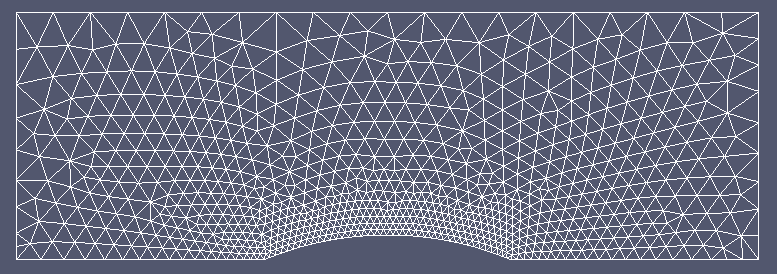
\includegraphics[width=1.0\linewidth]{bum_mesh_png}
		\caption{Mesh for the geometry internal flow past a bump}
	\end{figure}
	
	The current problem is not well-posed as there is no Dirichlet condition on $\phi$ and it will have multiple solutions or sometimes the solver can undergo convergence issues. To avoid this, $\phi$  is constrained to zero on one of the boundary nodes.\\
	Figure \ref{bum_phi} and \ref{bum_pres} shows the distribution of phi and pressure respectively. $\phi$ distribution shows that its contours are perpendicular at the walls as the normal velocities are zero and they are perpendicular to the streamlines as expected. From the pressure distribution, it can be observed that the pressure values are maximum at the bump corners when the velocities are minimum, and minimum at the top of the bump, when the velocities are maximum. This behavior is as expected because the energy is conserved in the system.
	
	\begin{figure}[h]\label{bum_phi}
		\centering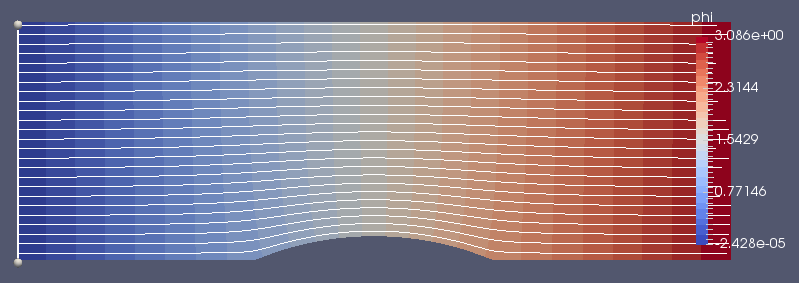
\includegraphics[width=1.0\linewidth]{bum_phi}
		\caption{Distribution of $\phi$ in internal flow past a bump}
	\end{figure}
	
	\begin{figure}[h]\label{bum_pres}
		\centering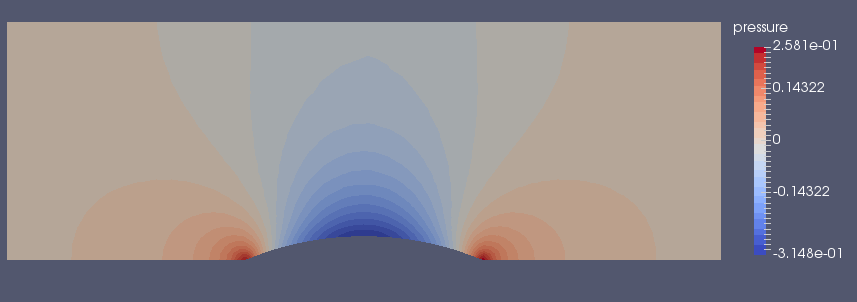
\includegraphics[width=1.0\linewidth]{bum_pres}
		\caption{Distribution of pressure in internal flow past a bump}
	\end{figure}
	
	Fig 5 shows the velocity distribution plot. The x component velocity is minimum at the corners because of the bent created by bump and maximum at the top as the cross-section is small. The freestream velocities are along x-direction but there is a small y component of velocities at the corners because of the bent. If the total magnitude of velocity is considered, it is minimum at the corners and maximum at the top because of the decreasing cross-section.
	
	
	\begin{figure}[h] \label{bum_vel}
		\centering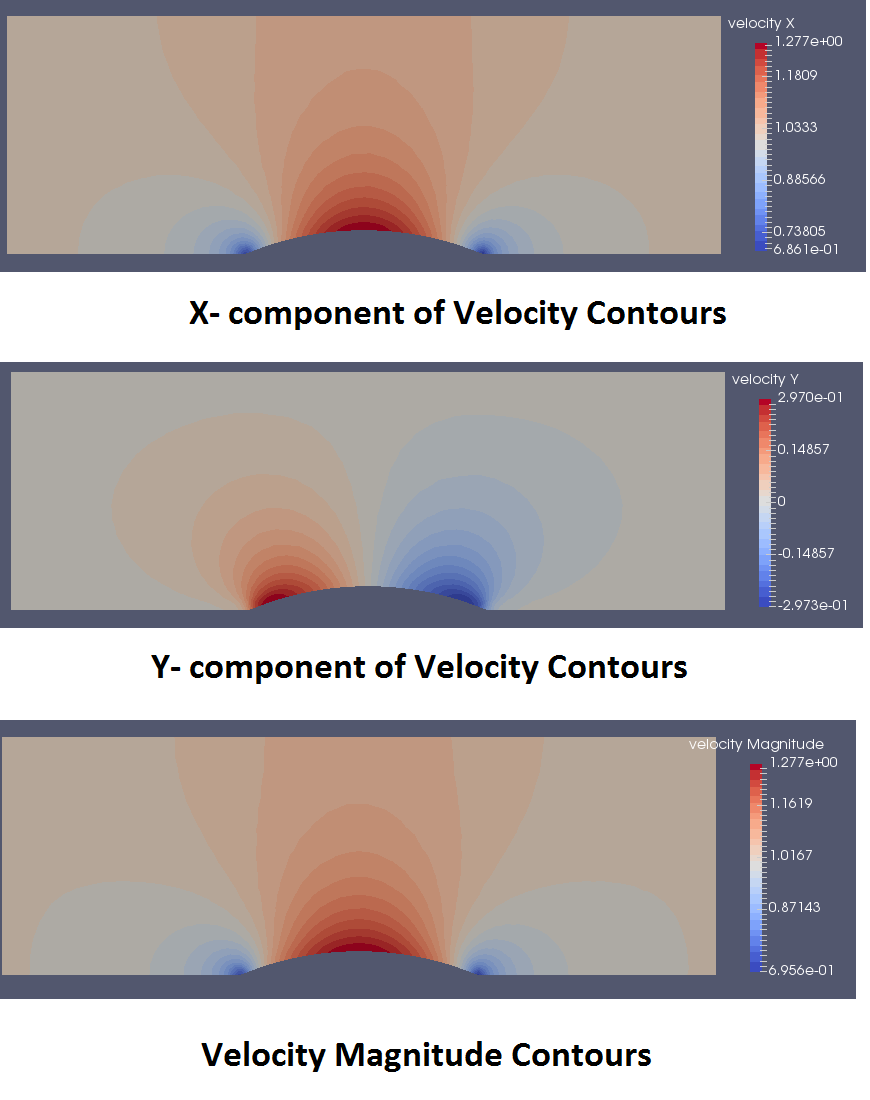
\includegraphics[width=1.0\linewidth]{figure_grid1_vel}
		\caption{Velocity distribution in internal flow past a bump}
	\end{figure}
	\clearpage
	
	\subsection{External flow past a cylinder}
	For external flow past a cylinder, Poisson’s equation is solved on four different meshes to understand the influence of mesh. Fig.6 shows the different grids used in this case. The boundary condition used in this problem is normal velocity is zero on the walls and on the far-field boundaries, a flux of $\phi$ ( g)=$(V_f,0).(nx,ny)$. Here $V_f$ is free to stream velocity and its value if one for this problem.
	
	\begin{figure}[h]\label{cylinder_grid}
		\centering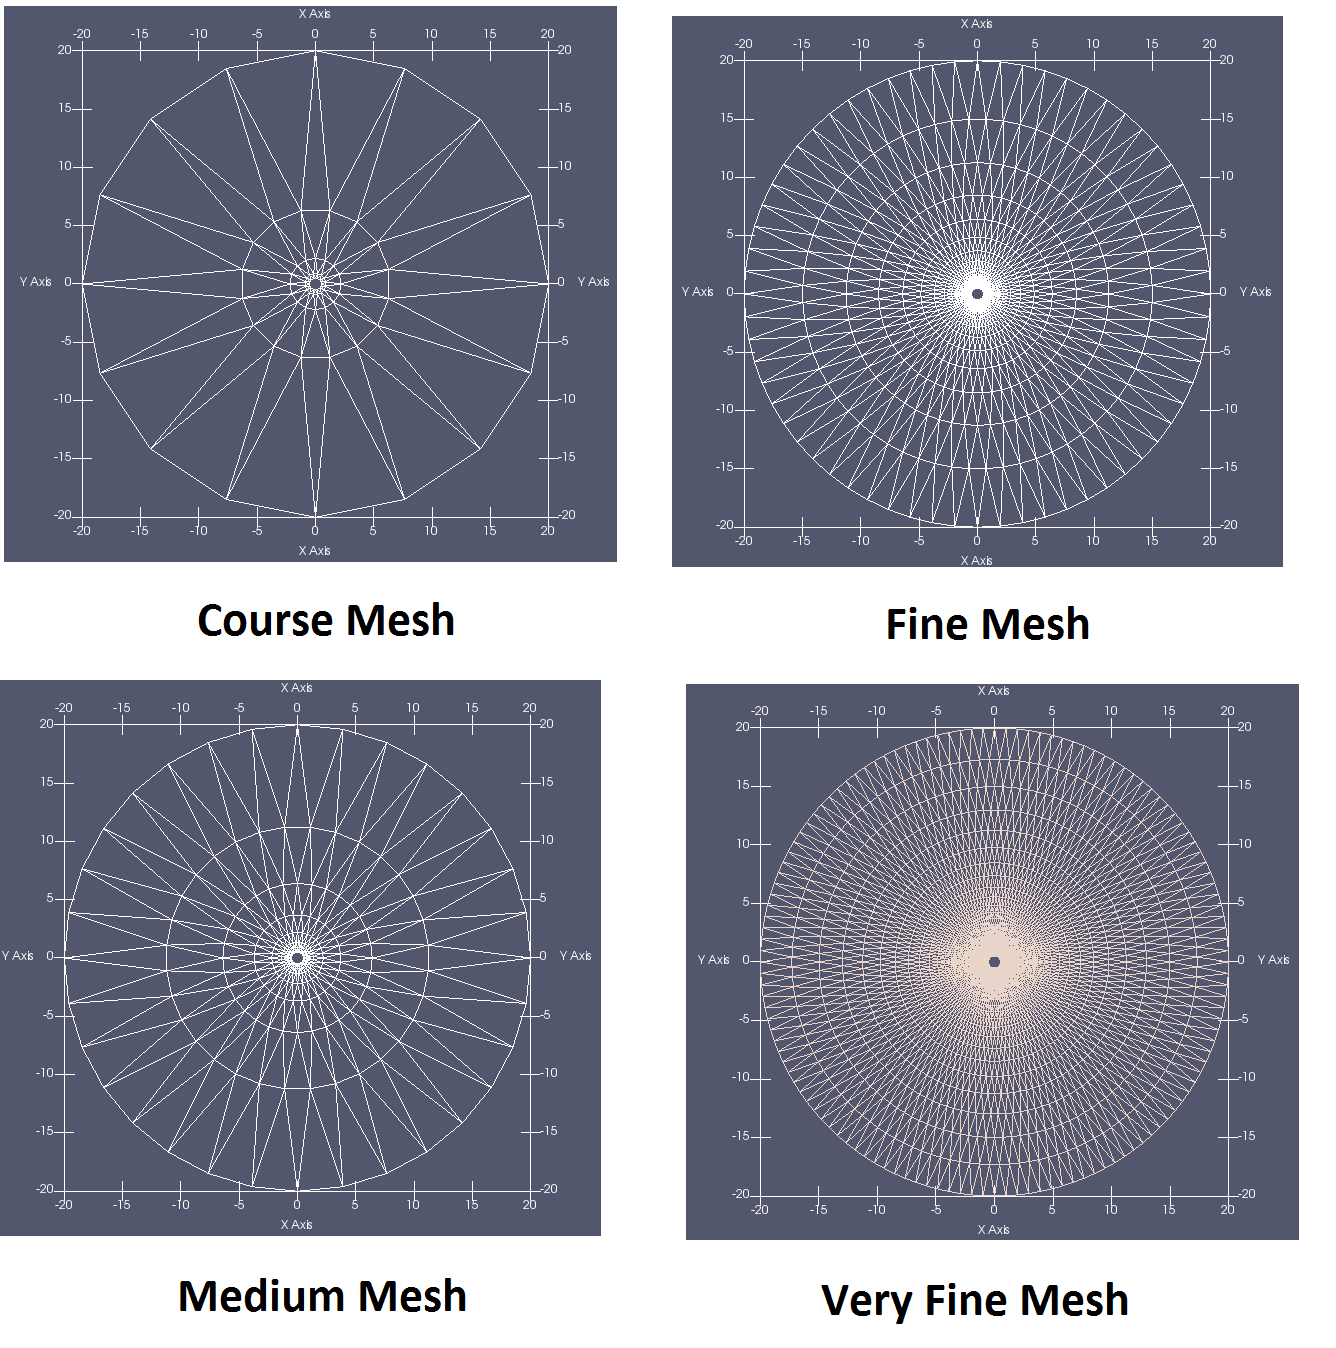
\includegraphics[width=1.0\linewidth]{figure_grid2}
		\caption{Different kind of meshes}
	\end{figure}
	
	Fig.7 and Fig. 8-11 show the distribution of phi and pressure respectively for flow past a cylinder. It can be observed that $\phi$ gradients are not resolved properly with a coarse mesh and well-resolved with fine mesh. This is evident from the pressure plot that the pressure contours are not smooth for coarse mesh and smoothness increases with an increase in mesh fineness. It can also be observed that absolute of maximum and minimum values of pressure is increasing with mesh refinement. 
	\begin{figure}[h] \label{cyl_phi}
		\centering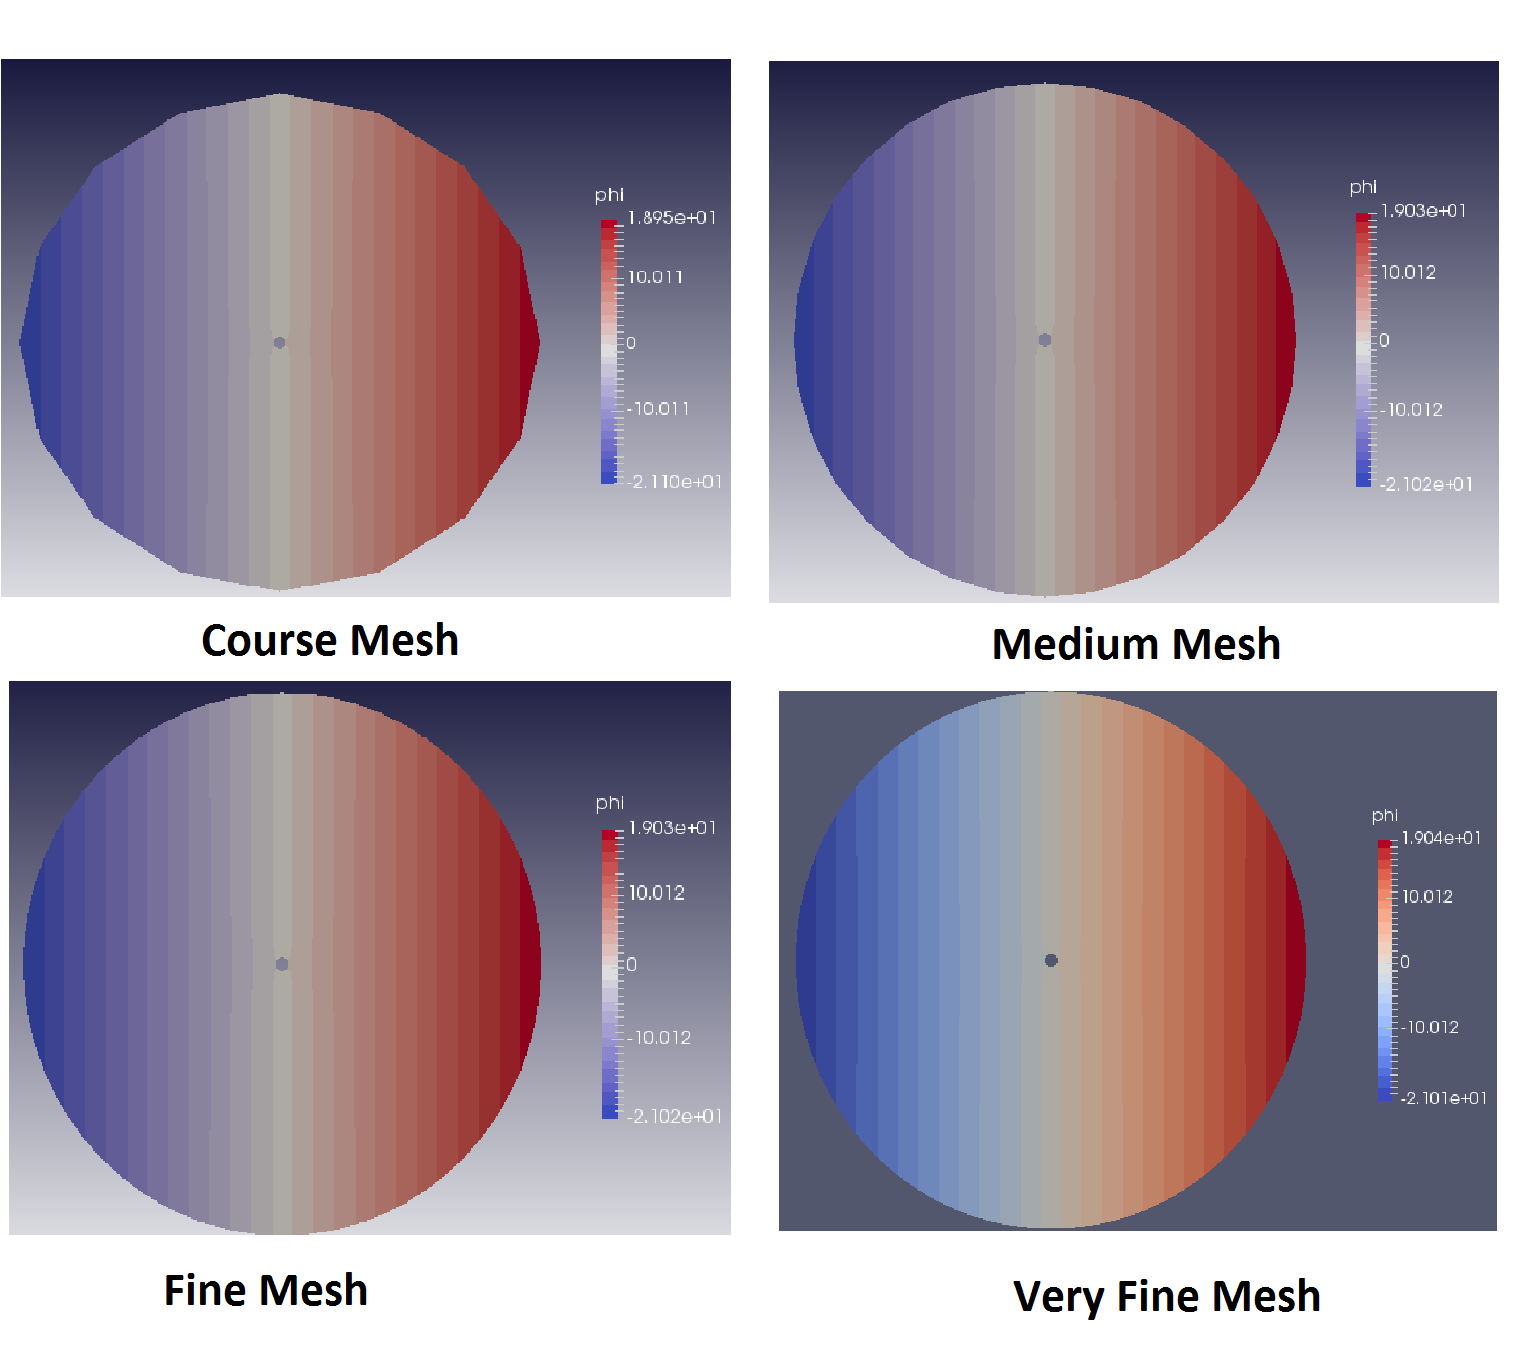
\includegraphics[width=1.0\linewidth]{figure_grid2_phi}
		\caption{Distribution of $\phi$ for external flow past a cylinder on different grids}
	\end{figure}
	
	\begin{figure}[h] \label{cyl__pres_cou}
		\centering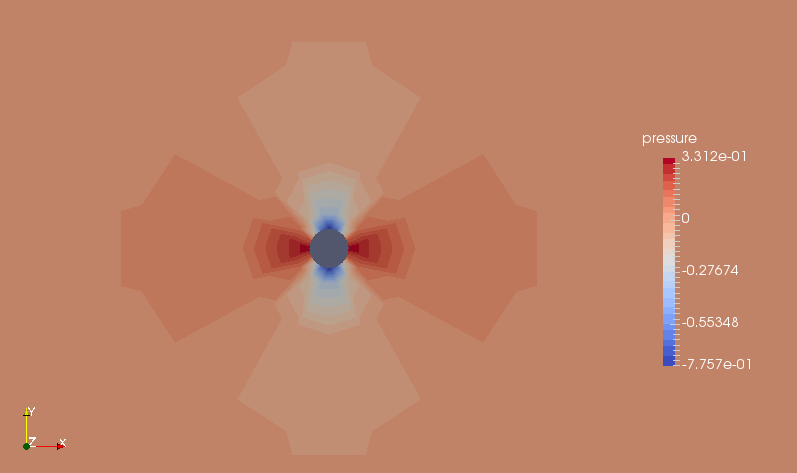
\includegraphics[width=1.0\linewidth]{pre_cou}
		\caption{Distribution of pressure for external flow past a cylinder on course grid}
	\end{figure}
	
	\begin{figure}[h] \label{cyl__pres_med}
		\centering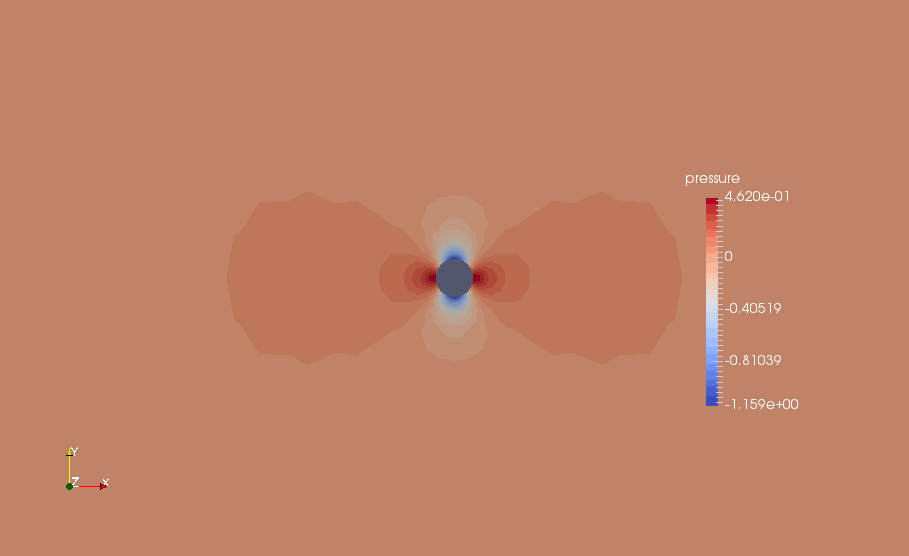
\includegraphics[width=1.0\linewidth]{pre_med}
		\caption{Distribution of pressure for external flow past a cylinder on medium grid}
	\end{figure}
	
	\begin{figure}[h] \label{cyl__pres_fin}
		\centering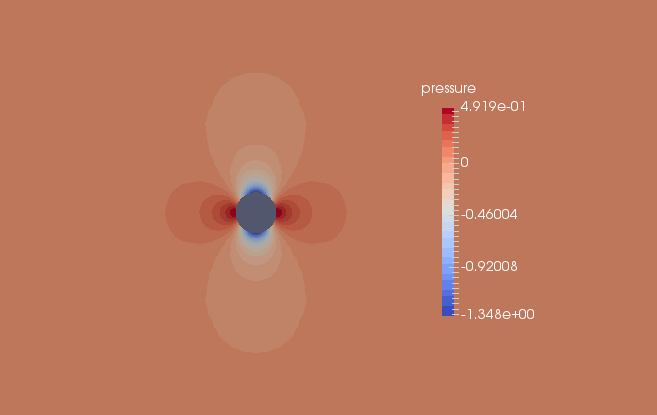
\includegraphics[width=1.0\linewidth]{pre_fin}
		\caption{Distribution of pressure for external flow past a cylinder on fine grid}
	\end{figure}
	\clearpage
	
	\begin{figure}[h] \label{cyl__pres_vfin}
		\centering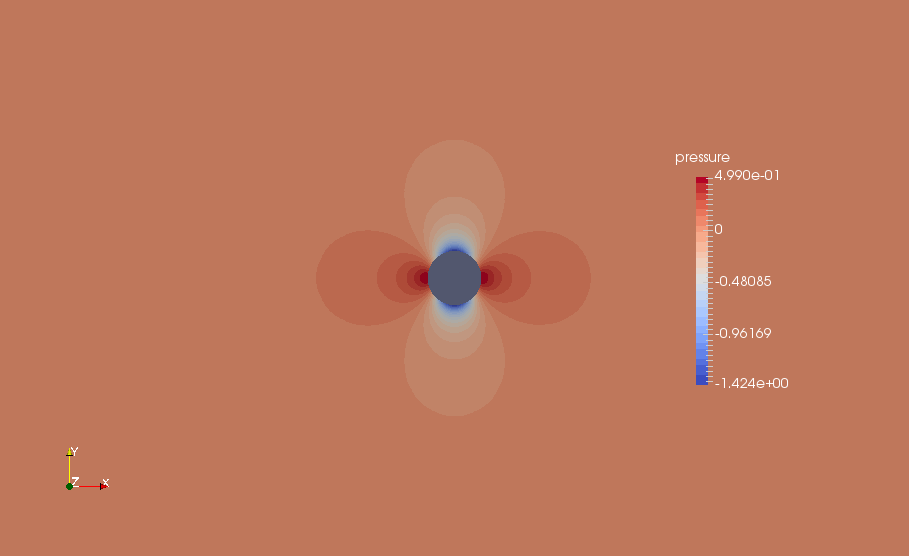
\includegraphics[width=1.0\linewidth]{pre_vfin}
		\caption{Distribution of pressure for external flow past a cylinder on very fine grid}
	\end{figure}
	
	Figs. 12-23 shows the distribution of x component, y-component and magnitude of velocity respectively. Velocities are following similar trend as that of pressure.
	\begin{figure}[h] \label{cyl__velx_cou}
		\centering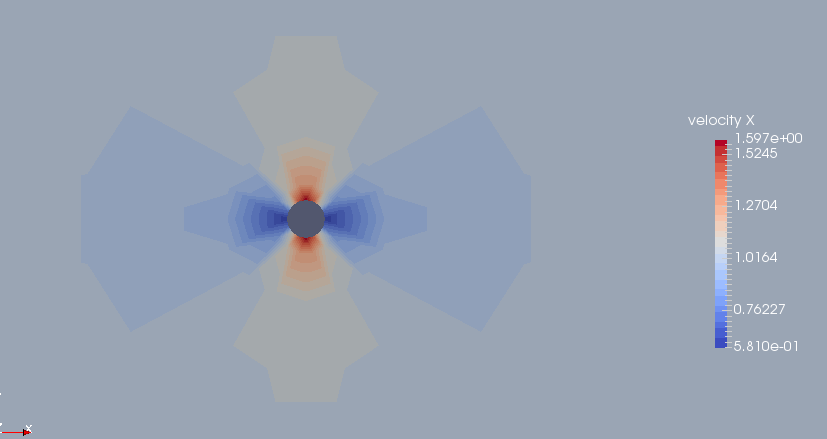
\includegraphics[width=1.0\linewidth]{velx_cou}
		\caption{Distribution of $v_x$ for external flow past a cylinder on course grid}
	\end{figure}
	
	\begin{figure}[h] \label{cyl__velx_med}
		\centering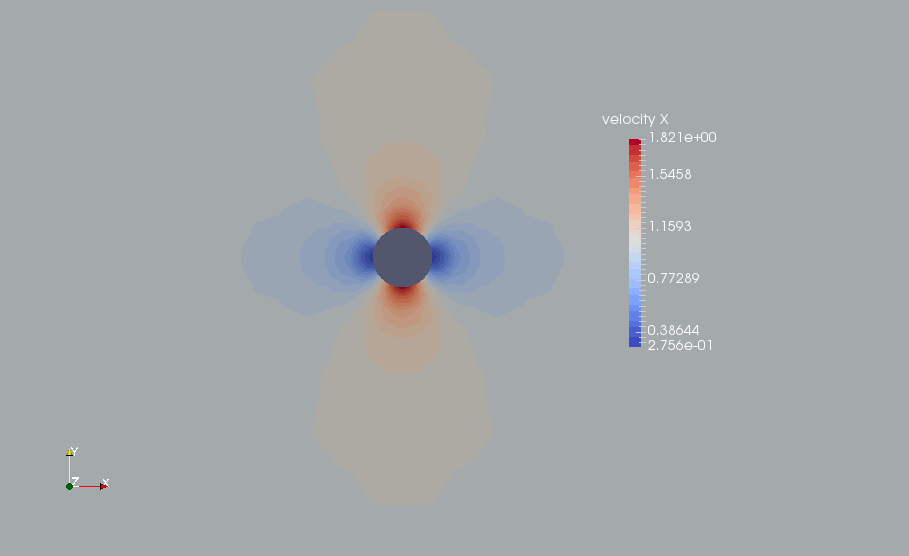
\includegraphics[width=1.0\linewidth]{velx_med}
		\caption{Distribution of $v_x$ for external flow past a cylinder on medium grid}
	\end{figure}
	
	\begin{figure}[h] \label{cyl__velx_fin}
		\centering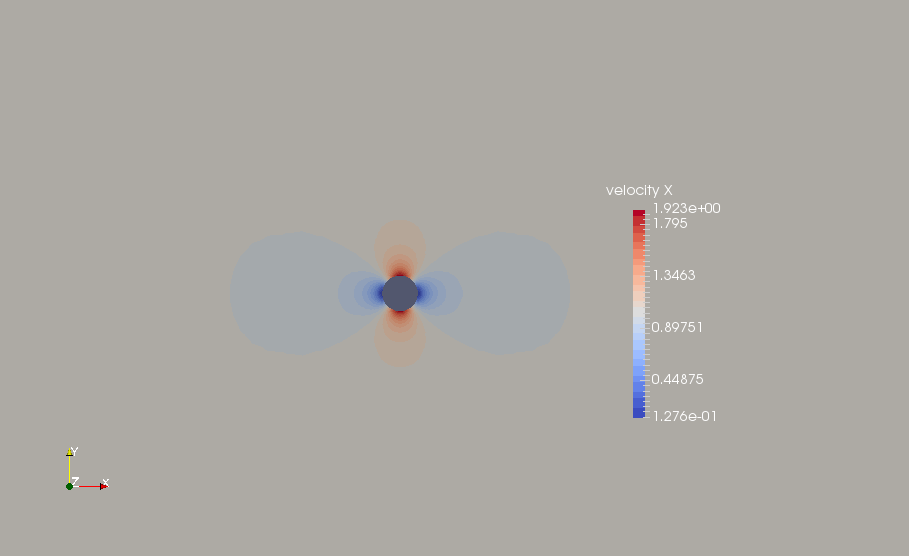
\includegraphics[width=1.0\linewidth]{velx_fin}
		\caption{Distribution of $v_x$ for external flow past a cylinder on fine grid}
	\end{figure}
	
	\begin{figure}[h] \label{cyl__velx_vfin}
		\centering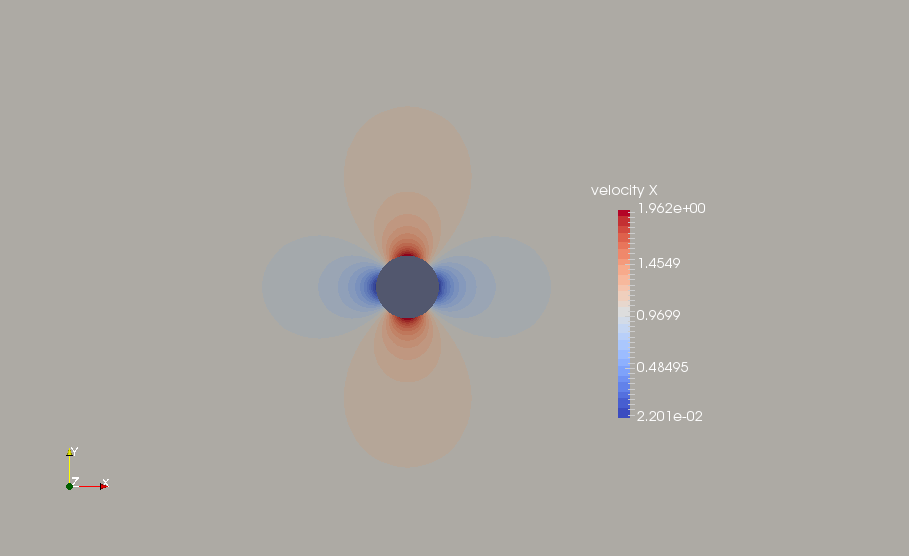
\includegraphics[width=1.0\linewidth]{velx_vfin}
		\caption{Distribution of $v_x$ for external flow past a cylinder on very fine grid}
	\end{figure}
	
	\begin{figure}[h] \label{cyl__vely_cou}
		\centering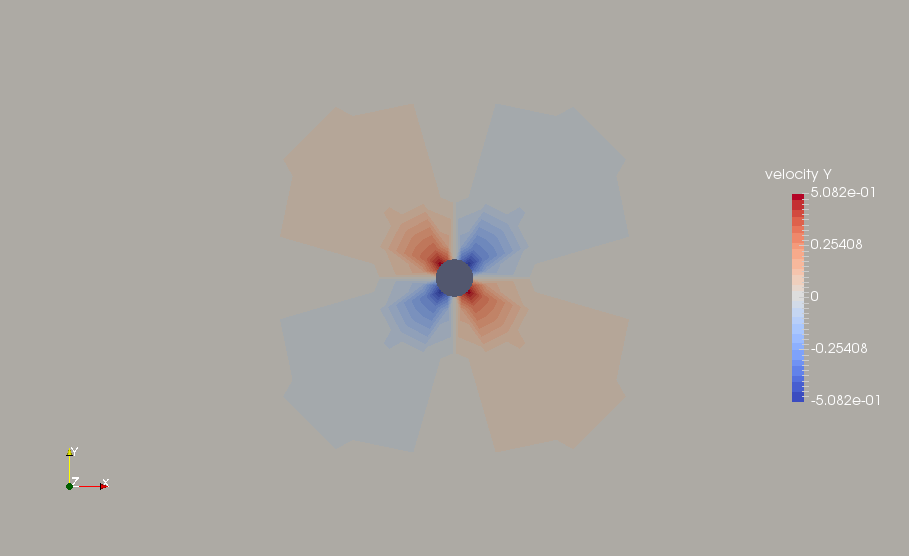
\includegraphics[width=1.0\linewidth]{vely_cou}
		\caption{Distribution of $v_y$ for external flow past a cylinder on course grid}
	\end{figure}
	
	\begin{figure}[h] \label{cyl__vely_med}
		\centering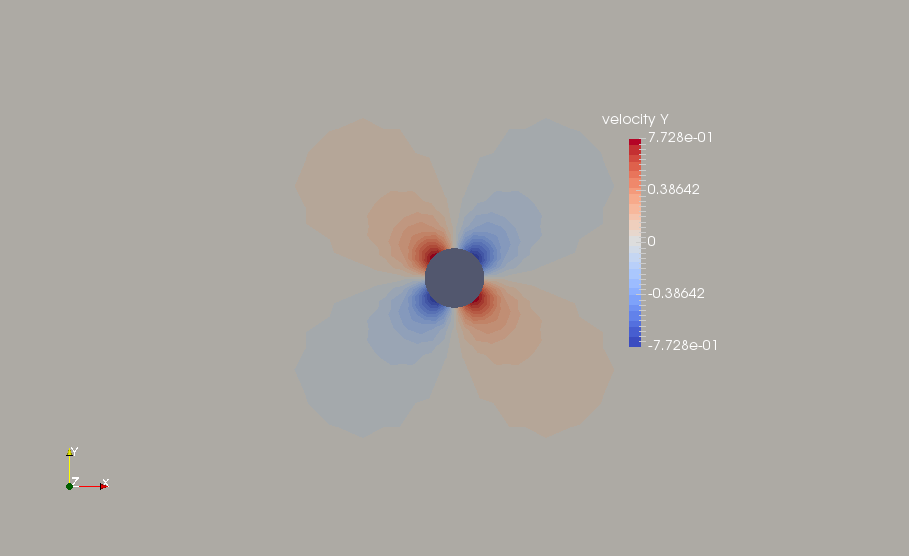
\includegraphics[width=1.0\linewidth]{vely_med}
		\caption{Distribution of $v_y$ for external flow past a cylinder on medium grid}
	\end{figure}
	
	\begin{figure}[h] \label{cyl__vely_fin}
		\centering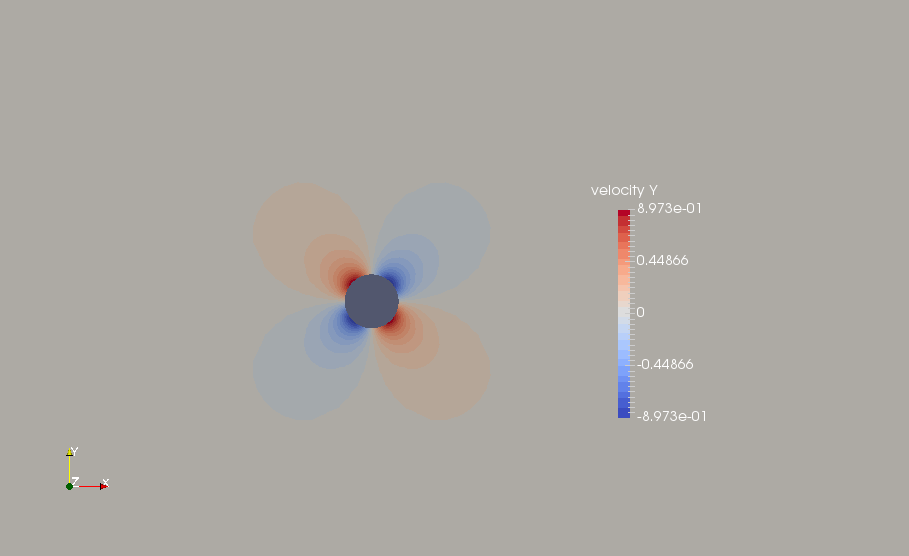
\includegraphics[width=1.0\linewidth]{vely_fin}
		\caption{Distribution of $v_y$ for external flow past a cylinder on fine grid}
	\end{figure}
	
	\begin{figure}[h] \label{cyl__vely_vfin}
		\centering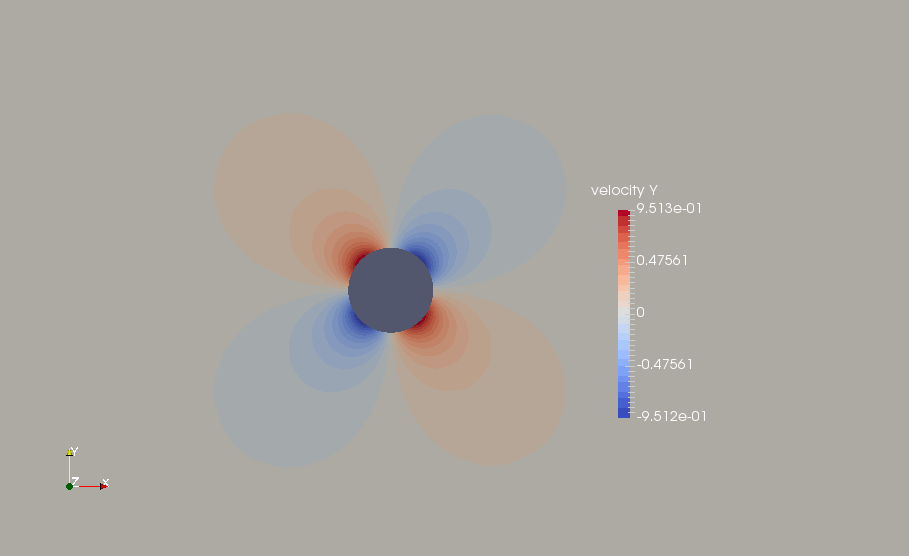
\includegraphics[width=1.0\linewidth]{vely_vfin}
		\caption{Distribution of $v_y$ for external flow past a cylinder on very fine grid}
	\end{figure}
	
	\begin{figure}[h] \label{cyl__velm_cou}
		\centering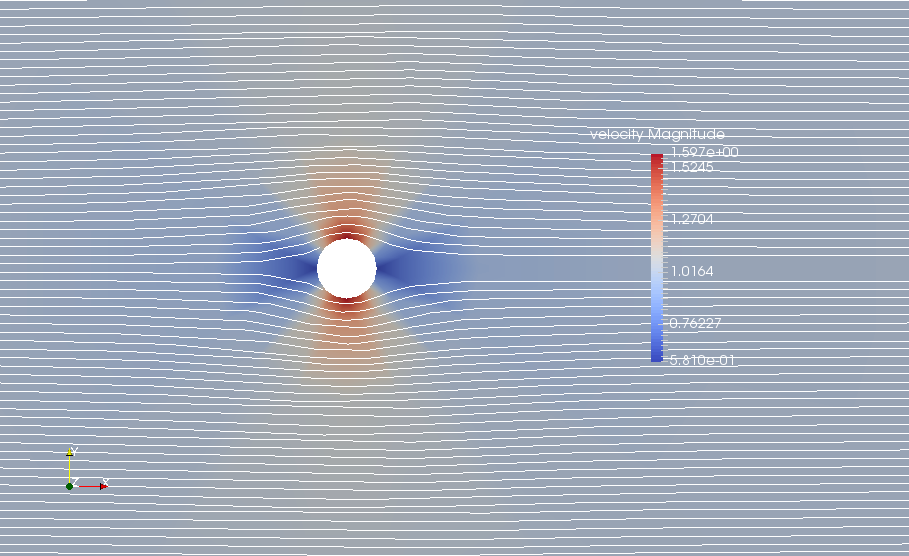
\includegraphics[width=1.0\linewidth]{velm_cou}
		\caption{Distribution of velocity magnitude for external flow past a cylinder on course grid}
	\end{figure}
	
	\begin{figure}[h] \label{cyl__velm_med}
		\centering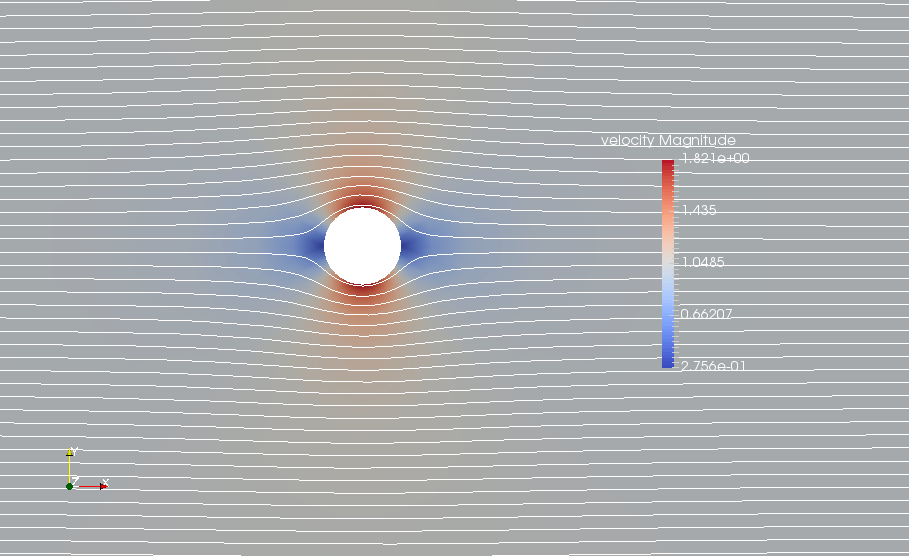
\includegraphics[width=1.0\linewidth]{velm_med}
		\caption{Distribution of velocity magnitude for external flow past a cylinder on medium grid}
	\end{figure}
	
	\begin{figure}[h] \label{cyl__velm_fin}
		\centering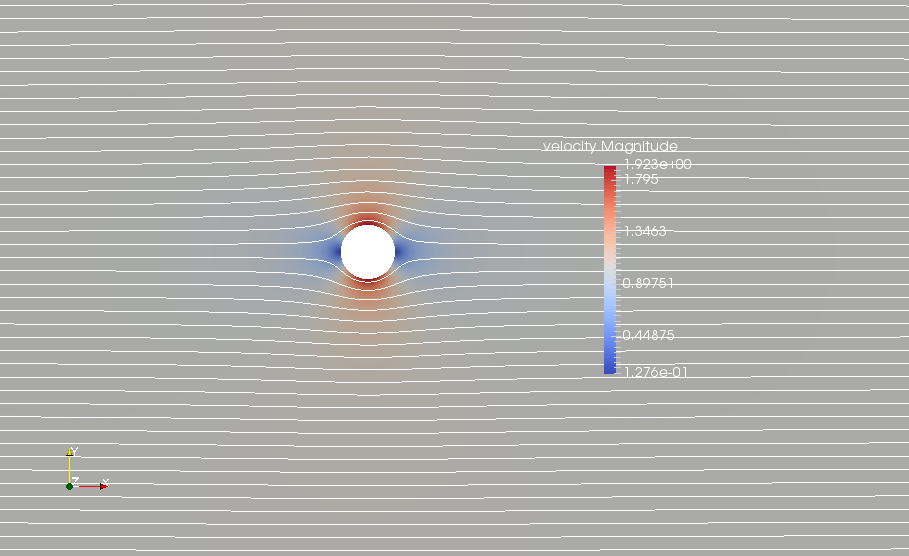
\includegraphics[width=1.0\linewidth]{velm_fin}
		\caption{Distribution of velocity magnitude for external flow past a cylinder on fine grid}
	\end{figure}
	
	\begin{figure}[h] \label{cyl__velm_vfin}
		\centering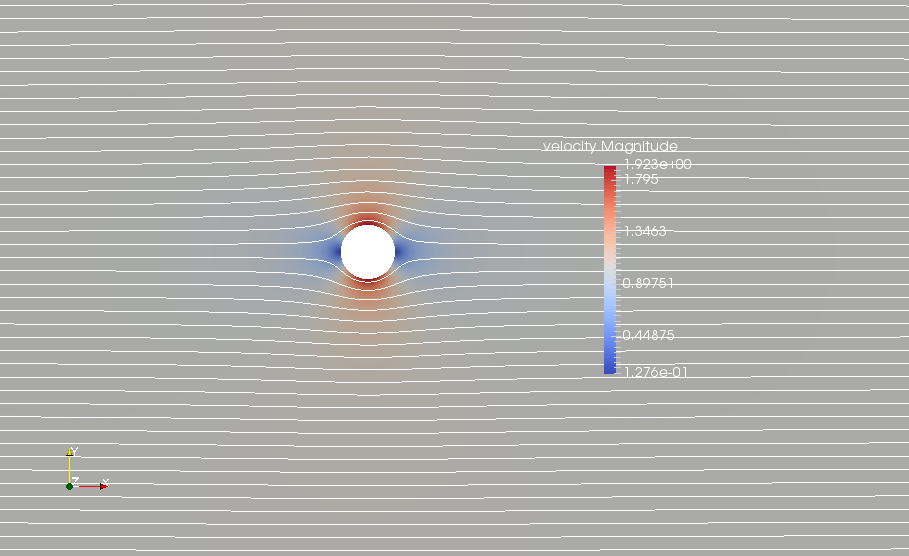
\includegraphics[width=1.0\linewidth]{velm_fin}
		\caption{Distribution of velocity magnitude for external flow past a cylinder on very fine grid}
	\end{figure}
	\clearpage
	
	From the above figures, it can be observed that the solution is well resolved using finer mesh and close to the theoretical values. If velocity magnitude distribution is considered, the values are closer to 0 at the coordinate points (-r,0) and (0,r) , which are also called stagnation points. The pressure values are maximum at the stagnation point and minimum at the top and bottom points of the cylinder.
	
	\subsection{Comparison of extern flow past a cylinder with exact solution}
	The exact solution for incompressible and irrational flow past a cylinder can be calculated using complex number theory. The exact solution in cylindrical coordinates is given by:
	
	\begin{equation}
		\begin{gathered}
			U_r=U(1-\frac{a^2}{r^2})cos(\theta) \\
			U_{\theta}=U(1+\frac{a^2}{r^2}) sin(\theta)
		\end{gathered}
	\end{equation}
	here a is the radius of the cylinder, U is the free stream velocity, and (r,$\theta$) is the coordinate system. For our problem, $a=0.5 m$ and $U=1 m/s$. The exact solution is calculated at the nodes of the mesh and the error function is defined by: E=$u_h-u_e$. Here $u_h$ is the numerical value at each node point and $u_e$ is the exact value at the node point. The average cell size is calculated by first calculating the elemental cell size by averaging over the nodes and that averaging over all elements. The norm of this error function will be of the form
	
	\begin{equation}
		||E||_{L^2}=C*h^{\alpha}
	\end{equation}
	The values of $||E||$ for each mesh is
	
	\begin{equation}
		\begin{gathered}
			h_avg \quad \quad ||E|| \\
			3.9414 \quad \quad 0.2528 \\
			1.9511 \quad \quad 0.3090 \\
			0.9731 \quad \quad 0.2803 \\
			0.4862 \quad \quad 0.2666 \\
		\end{gathered}
	\end{equation}
	
	Value for the coarse grid is completely offset compare to other girds and the reason is unknown. Plotted the values using the other three meshes.
	\clearpage
	\begin{figure}[h] \label{comp}
		\centering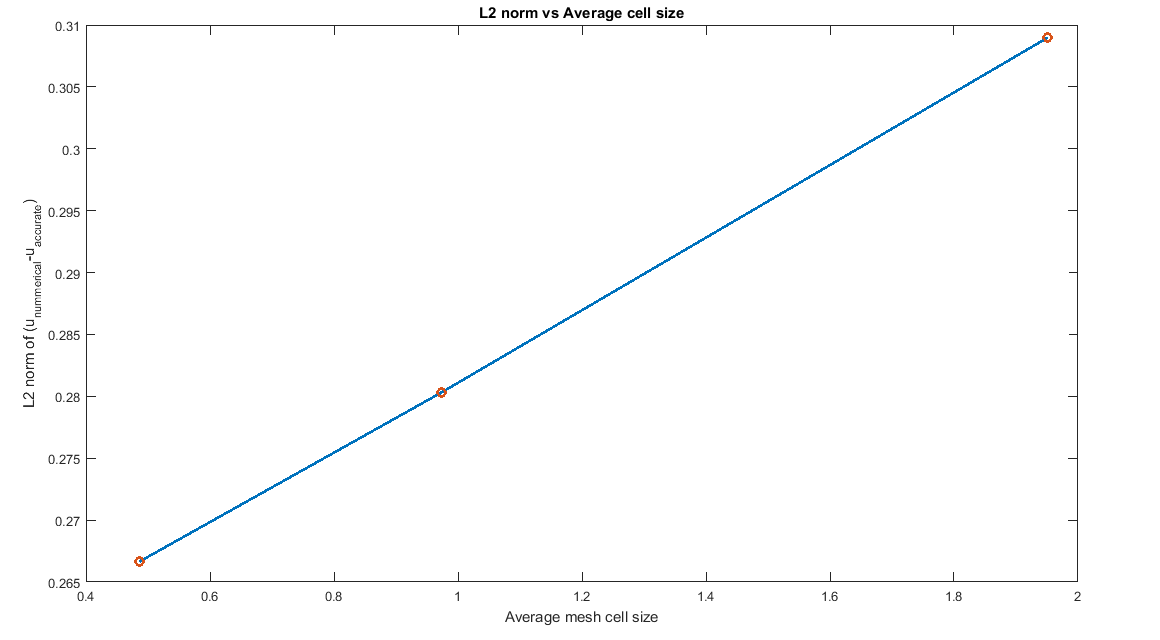
\includegraphics[width=1.0\linewidth]{comparisio}
		\caption{Distribution of velocity magnitude for external flow past a cylinder on course grid}
	\end{figure}
	The figure shows the plot is linear and the method used in this project is second-order accurate. This is because we are using linear elements.
	
	\section{Conclusion}
	In conclusion, the Finite element method is successfully implemented to solve the potential equation and tested in two cases. The solution for the first case, internal flow oven a bump, is matching with the theory, and grid mesh independent study is conducted on the external flow past a cylinder. From the mesh independent study it is found that the method used in this problem is first-order accurate because of using linear elements.
	
	%% The Appendices part is started with the command \appendix;
	%% appendix sections are then done as normal sections
	%% \appendix
	
	%% \section{}
	%% \label{}
	
	%% References
	%%
	%% Following citation commands can be used in the body text:
	%% Usage of \cite is as follows:
	%%   \cite{key}          ==>>  [#]
	%%   \cite[chap. 2]{key} ==>>  [#, chap. 2]
	%%   \citet{key}         ==>>  Author [#]
	
	%% References with bibTeX database:
	
	\bibliographystyle{model1-num-names}
	\bibliography{sample.bib}
	
	%% Authors are advised to submit their bibtex database files. They are
	%% requested to list a bibtex style file in the manuscript if they do
	%% not want to use model1-num-names.bst.
	
	%% References without bibTeX database:
	
	% \begin{thebibliography}{00}
	
	%% \bibitem must have the following form:
	%%   \bibitem{key}...
	%%
	
	% \bibitem{}
	
	% \end{thebibliography}
	
	
\end{document}

%%
%% End of file `elsarticle-template-1-num.tex'.
